\documentclass[11pt]{article}

\usepackage[utf8]{inputenc}
\usepackage[T1]{fontenc}
\usepackage[spanish]{babel}
\usepackage[margin=2.5cm]{geometry}
\usepackage{hyperref}
\usepackage{url}
\usepackage{booktabs}
\usepackage{multirow}
\usepackage{amsfonts}
\usepackage{amsmath}
\usepackage{amssymb}
\usepackage{nicefrac}
\usepackage{microtype}
\usepackage{graphicx}
\usepackage{subcaption}
\usepackage{float}
\usepackage{titling}
\usepackage{abstract}
\usepackage{xcolor}
\usepackage{listings}

\renewcommand{\abstractnamefont}{\normalfont\bfseries}
\renewcommand{\abstracttextfont}{\normalfont\small\itshape}

% --- Estilo para el codigo Python ---
\definecolor{codegreen}{rgb}{0.0,0.5,0.0}
\definecolor{codegray}{rgb}{0.5,0.5,0.5}
\definecolor{codepurple}{rgb}{0.58,0.0,0.82}
\definecolor{backcolour}{rgb}{0.96,0.96,0.94}

\lstdefinestyle{python}{
  backgroundcolor=\color{backcolour},
  commentstyle=\color{codegreen}\itshape,
  keywordstyle=\color{blue},
  stringstyle=\color{codepurple},
  basicstyle=\ttfamily\footnotesize,
  breakatwhitespace=false,
  breaklines=true,
  captionpos=b,
  keepspaces=true,
  numbers=left,
  numbersep=6pt,
  numberstyle=\tiny\color{codegray},
  showspaces=false,
  showstringspaces=false,
  showtabs=false,
  tabsize=4,
  frame=single,
  language=Python,
}
\lstset{style=python}

\graphicspath{{output/}}

\title{\textbf{TP 3 - Estudio de simulaci\'on de un sistema de colas
M/M/1}}

\author{
  Agustin Santinelli \\
  Ingenier\'ia en Sistemas de Informaci\'on \\
  Universidad Tecnol\'ogica Nacional \\
  Legajo 52211 \\
  \texttt{agustinsantinelli@gmail.com}
  \and
  Joaquin Peralta \\
  Ingenier\'ia en Sistemas de Informaci\'on \\
  Universidad Tecnol\'ogica Nacional \\
  Legajo 52151 \\
  \texttt{joaaperalta@gmail.com}
  \and
  Martin Ratti \\
  Ingenier\'ia en Sistemas de Informaci\'on \\
  Universidad Tecnol\'ogica Nacional \\
  Legajo 52398 \\
  \texttt{martinratti10@gmail.com}
  \and
  Tomas Levrand \\
  Ingenier\'ia en Sistemas de Informaci\'on \\
  Universidad Tecnol\'ogica Nacional \\
  Legajo 52206 \\
  \texttt{tomylevrand@gmail.com}
}

\date{\today}

\begin{document}
\maketitle

\begin{abstract}
\noindent Se construye un simulador de eventos discretos del sistema de
colas M/M/1 (y su variante de capacidad finita M/M/1/K) y se contrasta su
salida contra la teor\'ia cl\'asica de colas markovianas. Sobre el motor de
avance al pr\'oximo evento se miden las medidas de rendimiento usuales ---
n\'umero medio de clientes en el sistema $L$ y en la cola $L_q$, tiempo
medio en el sistema $W$ y de espera $W_q$, utilizaci\'on del servidor, la
distribuci\'on estacionaria $P_n$ y la probabilidad de denegaci\'on de
servicio --- variando la intensidad de tr\'afico $\rho$ en
$\{25, 50, 75, 100, 125\}\%$ y, para la cola finita, la capacidad $K$ en
$\{0, 2, 5, 10, 50\}$. Cada experimento se replica $10$ veces con semillas
independientes y se reporta su intervalo de confianza al $95\%$. La fuente
de aleatoriedad es el Generador Congruencial Lineal validado en el TP 2.1,
del que se obtienen los tiempos exponenciales por transformaci\'on inversa.
Los resultados confirman que, en r\'egimen estable ($\rho < 1$), las medidas
simuladas reproducen las te\'oricas con error menor al $2\%$, y que la cola
finita permite estudiar tambi\'en los reg\'imenes saturados
($\rho \ge 1$). El estudio contrasta \emph{tres} fuentes de datos
independientes --- te\'orico, Python y AnyLogic --- que concuerdan entre s\'i,
validando el modelo desde tres perspectivas complementarias.

\vspace{0.5em}
\noindent\textbf{Palabras clave:} Simulaci\'on, Eventos discretos, Teor\'ia
de colas, M/M/1, M/M/1/K, Ley de Little, Probabilidad de denegaci\'on,
Intervalo de confianza.
\end{abstract}

\section{Introducci\'on}

Un sistema de colas modela el flujo de \emph{clientes} que arriban a un
\emph{servidor}, eventualmente esperan en una \emph{cola} y son atendidos.
La cola \textbf{M/M/1} es el caso can\'onico: un \'unico servidor, arribos
\emph{poissonianos} y tiempos de servicio \emph{exponenciales}. Su inter\'es
radica en que, pese a su simplicidad, admite soluci\'on anal\'itica cerrada
y por eso sirve de banco de pruebas ideal para validar un simulador de
eventos discretos: todo lo que el simulador estime puede contrastarse contra
una f\'ormula exacta.

\subsection{Notaci\'on de Kendall}

La notaci\'on de Kendall \verb|A/B/c/K| describe un sistema de colas por su
proceso de arribos $A$, su distribuci\'on de servicio $B$, el n\'umero de
servidores $c$ y la capacidad m\'axima $K$. En \textbf{M/M/1}, la primera
\textbf{M} (\emph{markoviano}) indica arribos de Poisson --- tiempos entre
arribos exponenciales ---; la segunda \textbf{M}, servicio exponencial; y el
\textbf{1}, un \'unico servidor. Cuando se omite $K$ la capacidad es
infinita. La variante \textbf{M/M/1/K} agrega una capacidad m\'axima $K$:
un arribo que encuentra el sistema con $K$ clientes es \emph{rechazado}
(denegaci\'on de servicio).

\subsection{Supuestos del modelo}

El modelo descansa sobre cuatro supuestos:
\begin{itemize}
  \item \textbf{Arribos Poisson:} los tiempos entre arribos son
    exponenciales independientes de tasa $\lambda$.
  \item \textbf{Servicio exponencial:} los tiempos de servicio son
    exponenciales independientes de tasa $\mu$.
  \item \textbf{Un servidor:} existe una \'unica estaci\'on de atenci\'on.
  \item \textbf{Disciplina FIFO:} se atiende en orden de llegada
    (\emph{first in, first out}).
\end{itemize}

\subsection{Fuente de aleatoriedad}

Toda la aleatoriedad del simulador proviene del Generador Congruencial
Lineal (GCL) validado en el TP 2.1 (configuraci\'on \texttt{MINSTD}:
$a = 48271$, $c = 0$, $m = 2^{31}-1$), reutilizado aqu\'i como fuente de
uniformes $U \sim U(0,1)$. Los tiempos exponenciales --- entre arribos y de
servicio --- se obtienen de esos uniformes por \emph{transformaci\'on
inversa}: dado que la acumulada exponencial de tasa $r$ es
$F(x) = 1 - e^{-rx}$, despejando se llega a
\begin{equation}
x = -\frac{\ln U}{r},
\end{equation}
con $U \in (0,1)$. Cada r\'eplica usa una semilla distinta del GCL para
garantizar corridas independientes.

\lstinputlisting[caption={Fuente de uniformes: GCL reutilizado del TP 2.1
(\texttt{cola/rng.py}).}, label={lst:rng}]{codigo/rng.py}

\section{Marco te\'orico y f\'ormulas}

\subsection{Intensidad de tr\'afico y estabilidad}

La \emph{intensidad de tr\'afico} o \emph{utilizaci\'on} del servidor es el
cociente entre la tasa de arribos y la de servicio:
\begin{equation}
\rho = \frac{\lambda}{\mu}.
\end{equation}
Para la cola \textbf{infinita}, la \emph{condici\'on de estabilidad} es
\begin{equation}
\rho < 1,
\end{equation}
es decir, que en promedio el servidor pueda despachar clientes m\'as r\'apido
de lo que llegan. Si $\rho \ge 1$ el sistema es \emph{inestable}: la cola
crece sin cota y no existe distribuci\'on estacionaria.

\subsection{Medidas de rendimiento (cola infinita)}

Bajo estabilidad, las medidas de rendimiento de la M/M/1 tienen forma
cerrada. El n\'umero medio de clientes en el sistema y en la cola son
\begin{equation}
L = \frac{\rho}{1-\rho},
\qquad
L_q = \frac{\rho^2}{1-\rho}.
\end{equation}
Los tiempos medios en el sistema y de espera en la cola son
\begin{equation}
W = \frac{1}{\mu-\lambda},
\qquad
W_q = \frac{\rho}{\mu-\lambda}.
\end{equation}
La distribuci\'on estacionaria del n\'umero de clientes es geom\'etrica:
\begin{equation}
P_n = (1-\rho)\,\rho^{\,n},
\qquad n = 0, 1, 2, \dots
\end{equation}

\subsection{Ley de Little}

La \emph{ley de Little} vincula los promedios espaciales (clientes) con los
temporales (tiempos) a trav\'es de la tasa de arribos, sin suponer ninguna
distribuci\'on en particular:
\begin{equation}
L = \lambda\,W,
\qquad
L_q = \lambda\,W_q.
\end{equation}
Por su generalidad, se usa en este trabajo como \emph{verificaci\'on
cruzada}: las cuatro medidas estimadas deben satisfacerla.

\subsection{Cola finita M/M/1/K}

Cuando la capacidad es finita el sistema admite a lo sumo $K$ clientes. La
distribuci\'on estacionaria existe \emph{siempre} (la capacidad acota el
sistema, incluso con $\rho \ge 1$) y vale
\begin{equation}
P_n =
\begin{cases}
\dfrac{\rho^{\,n}\,(1-\rho)}{1-\rho^{\,K+1}}, & \rho \neq 1, \\[1.2em]
\dfrac{1}{K+1}, & \rho = 1,
\end{cases}
\qquad 0 \le n \le K.
\end{equation}
La \emph{probabilidad de denegaci\'on} (o de bloqueo) es la probabilidad de
que un arribo encuentre el sistema lleno, es decir $P_K$:
\begin{equation}
P_{\text{deneg}} = P_K.
\end{equation}
Como una fracci\'on $P_K$ de los arribos se rechaza, la tasa de arribos
\emph{efectiva} (clientes que realmente entran) es
\begin{equation}
\lambda_{\text{ef}} = \lambda\,(1 - P_K),
\end{equation}
y es esta tasa efectiva la que debe usarse en la ley de Little para la cola
finita: $L = \lambda_{\text{ef}}\,W$ y $L_q = \lambda_{\text{ef}}\,W_q$.

\section{Metodolog\'ia}

\subsection{Simulaci\'on de eventos discretos}

El simulador implementa el esquema de \emph{avance al pr\'oximo evento}
(\emph{next-event time-advance}) descrito en Law \cite{law}, cap\'itulo 1.
En lugar de avanzar el tiempo a pasos fijos, el reloj salta directamente al
instante del pr\'oximo evento relevante. El modelo tiene s\'olo \emph{dos}
tipos de evento:
\begin{itemize}
  \item \textbf{Arribo:} llega un cliente. Si la cola no est\'a llena, entra
    (al servidor si est\'a libre, o a la cola FIFO si no). Se programa el
    pr\'oximo arribo. En la variante finita, si el sistema ya tiene $K$
    clientes, el arribo se rechaza y se contabiliza como denegaci\'on.
  \item \textbf{Partida:} un cliente termina su servicio y abandona el
    sistema. Si hay clientes esperando, el primero de la cola pasa a
    servicio; si no, el servidor queda ocioso.
\end{itemize}
En cada iteraci\'on, el pr\'oximo evento es el de menor tiempo entre el
arribo y la partida programados, y el reloj avanza hasta \'el.

\subsection{Estimaci\'on de las medidas}

Los promedios \emph{temporales} ($L$ y $L_q$) se obtienen \emph{integrando
las \'areas} bajo las funciones escalera $L(t)$ y $Q(t)$. Entre dos eventos
consecutivos el n\'umero de clientes es constante, de modo que el \'area se
acumula exactamente como $\text{n\_clientes} \times \Delta t$ (regla del
rect\'angulo, exacta para funciones escalera). Al final se divide por el
horizonte total:
\begin{equation}
L = \frac{1}{T}\int_0^{T} L(t)\,dt,
\qquad
L_q = \frac{1}{T}\int_0^{T} Q(t)\,dt.
\end{equation}
Los promedios \emph{por cliente} ($W$ y $W_q$) se estiman acumulando, para
cada cliente atendido, su tiempo en el sistema (instante de partida menos
instante de arribo) y su tiempo de espera en cola, y dividiendo por la
cantidad de clientes atendidos. La \emph{utilizaci\'on observada} es la
fracci\'on de tiempo con el servidor ocupado,
\begin{equation}
\hat{\rho} = \frac{\text{busy\_time}}{T},
\end{equation}
y la \emph{probabilidad de denegaci\'on} es el cociente entre arribos
rechazados y arribos totales. La distribuci\'on $P_n$ se estima como la
fracci\'on de tiempo que el sistema pasa con exactamente $n$ clientes.

\subsection{R\'eplicas e intervalos de confianza}

Cada experimento se corre con $10$ r\'eplicas independientes (semillas
distintas del GCL), $\mu = 1$ y horizonte $T = 5000$. Para cada medida se
reporta la media de las r\'eplicas y su \emph{intervalo de confianza al
$95\%$}, calculado con la $t$ de Student a $n-1 = 9$ grados de libertad:
\begin{equation}
\bar{x} \pm t_{0{,}975,\,9}\;\frac{s}{\sqrt{n}},
\end{equation}
donde $\bar{x}$ y $s$ son la media y el desv\'io muestrales entre r\'eplicas.

\subsection{C\'odigo de la simulaci\'on}

El n\'ucleo del motor es el lazo de eventos, que avanza el reloj, acumula
las \'areas y procesa arribos y partidas:

\lstinputlisting[firstline=160, lastline=237, caption={Lazo de eventos del
motor de simulaci\'on (\texttt{cola/simulacion.py}): avance al pr\'oximo
evento, integraci\'on de \'areas y procesamiento de arribos/partidas.},
label={lst:loop}]{codigo/simulacion.py}

Al terminar el horizonte, los estimadores finales se obtienen normalizando
los acumuladores:

\lstinputlisting[firstline=238, lastline=249, caption={C\'alculo de los
estimadores finales: $L$, $L_q$, $\hat{\rho}$, $W$, $W_q$, probabilidad de
denegaci\'on y distribuci\'on $P_n$.}]{codigo/simulacion.py}

Las f\'ormulas te\'oricas contra las que se contrasta se implementan en un
m\'odulo aparte. Para la cola infinita:

\lstinputlisting[firstline=71, lastline=112, caption={F\'ormulas te\'oricas
de la cola M/M/1 infinita (\texttt{cola/teorico.py}). Si $\rho \ge 1$ las
medidas divergen y se marca el sistema como inestable.}]{codigo/teorico.py}

Y para la cola finita M/M/1/K, donde las medidas temporales usan la tasa de
arribos efectiva:

\lstinputlisting[firstline=132, lastline=183, caption={F\'ormulas te\'oricas
de la cola M/M/1/K finita (\texttt{cola/teorico.py}): siempre estable, con
probabilidad de bloqueo $P_K$ y tasa efectiva
$\lambda_{\text{ef}}$.}]{codigo/teorico.py}

\section{Resultados}

\subsection{M/M/1 infinita: simulado vs.\ te\'orico}

La Tabla~\ref{tab:infinita} compara, para cada nivel de carga $\rho$, las
medidas simuladas (media e intervalo de confianza al $95\%$ sobre $10$
r\'eplicas) contra las te\'oricas, con el error relativo. En la zona estable
($\rho \in \{0{,}25,\,0{,}50,\,0{,}75\}$) el error es siempre menor al $2\%$
y el intervalo de confianza contiene al valor te\'orico. Para
$\rho \ge 1$ el sistema infinito es \emph{inestable}: el valor te\'orico es
infinito, y lo que se reporta es el valor simulado, que crece sin l\'imite y
s\'olo queda acotado por el horizonte finito $T = 5000$.

\begin{table}[H]
\centering
\small
\begin{tabular}{llrrr}
\toprule
\textbf{$\rho$} & \textbf{Medida} & \textbf{Simulado (media [IC95])}
& \textbf{Te\'orico} & \textbf{Error} \\
\midrule
\multirow{5}{*}{$0{,}25$}
 & $L$           & $0{,}3365$ \, [$0{,}324$--$0{,}349$] & $0{,}3333$ & $0{,}94\%$ \\
 & $L_q$         & $0{,}0847$ \, [$0{,}077$--$0{,}092$] & $0{,}0833$ & $1{,}61\%$ \\
 & $W$           & $1{,}3260$ \, [$1{,}283$--$1{,}369$] & $1{,}3333$ & $0{,}55\%$ \\
 & $W_q$         & $0{,}3335$ \, [$0{,}307$--$0{,}360$] & $0{,}3333$ & $0{,}04\%$ \\
 & $\hat{\rho}$  & $0{,}2518$                           & $0{,}2500$ & $0{,}71\%$ \\
\midrule
\multirow{5}{*}{$0{,}50$}
 & $L$           & $1{,}0020$ \, [$0{,}983$--$1{,}021$] & $1{,}0000$ & $0{,}20\%$ \\
 & $L_q$         & $0{,}5032$ \, [$0{,}486$--$0{,}520$] & $0{,}5000$ & $0{,}65\%$ \\
 & $W$           & $2{,}0019$ \, [$1{,}958$--$2{,}045$] & $2{,}0000$ & $0{,}10\%$ \\
 & $W_q$         & $1{,}0054$ \, [$0{,}971$--$1{,}040$] & $1{,}0000$ & $0{,}54\%$ \\
 & $\hat{\rho}$  & $0{,}4988$                           & $0{,}5000$ & $0{,}25\%$ \\
\midrule
\multirow{5}{*}{$0{,}75$}
 & $L$           & $2{,}9631$ \, [$2{,}810$--$3{,}116$] & $3{,}0000$ & $1{,}23\%$ \\
 & $L_q$         & $2{,}2146$ \, [$2{,}066$--$2{,}363$] & $2{,}2500$ & $1{,}57\%$ \\
 & $W$           & $3{,}9442$ \, [$3{,}753$--$4{,}135$] & $4{,}0000$ & $1{,}40\%$ \\
 & $W_q$         & $2{,}9473$ \, [$2{,}760$--$3{,}135$] & $3{,}0000$ & $1{,}76\%$ \\
 & $\hat{\rho}$  & $0{,}7485$                           & $0{,}7500$ & $0{,}20\%$ \\
\midrule
\multirow{5}{*}{$1{,}00$}
 & $L$           & $52{,}47$  & $\infty$ & --- \\
 & $L_q$         & $51{,}49$  & $\infty$ & --- \\
 & $W$           & $52{,}30$  & $\infty$ & --- \\
 & $W_q$         & $51{,}32$  & $\infty$ & --- \\
 & $\hat{\rho}$  & $0{,}9850$ & $1{,}0000$ & --- \\
\midrule
\multirow{5}{*}{$1{,}25$}
 & $L$           & $613{,}22$ & $\infty$ & --- \\
 & $L_q$         & $612{,}22$ & $\infty$ & --- \\
 & $W$           & $491{,}42$ & $\infty$ & --- \\
 & $W_q$         & $490{,}62$ & $\infty$ & --- \\
 & $\hat{\rho}$  & $0{,}9995$ & $1{,}0000$ & --- \\
\bottomrule
\end{tabular}
\caption{Cola M/M/1 infinita: medidas simuladas (media e IC al $95\%$ sobre
$10$ r\'eplicas, $\mu = 1$, $T = 5000$) vs.\ te\'oricas. Para
$\rho \ge 1$ el sistema es inestable: el valor te\'orico es infinito y el
simulado s\'olo queda acotado por el horizonte finito.}
\label{tab:infinita}
\end{table}

\subsection{M/M/1/K: probabilidad de denegaci\'on}

La Tabla~\ref{tab:denegacion} reporta la probabilidad de denegaci\'on
simulada y te\'orica para cada combinaci\'on de carga $\rho$ y capacidad
$K \in \{0,\,2,\,5,\,10,\,50\}$. Con $K = 0$ (sin sala de espera) todo
arribo que encuentra el servidor ocupado se rechaza, por lo que la
denegaci\'on es total bajo carga. A medida que crece $K$ la denegaci\'on
decae, y crece con la carga $\rho$.

\begin{table}[H]
\centering
\small
\begin{tabular}{lrrrrr}
\toprule
\textbf{$\rho$} & \textbf{$K=0$} & \textbf{$K=2$} & \textbf{$K=5$}
& \textbf{$K=10$} & \textbf{$K=50$} \\
 & sim/te\'o & sim/te\'o & sim/te\'o & sim/te\'o & sim/te\'o \\
\midrule
$0{,}25$ & $1{,}00000$/$1{,}00000$ & $0{,}04947$/$0{,}04762$
         & $0{,}00070$/$0{,}00073$ & ${\sim}0$/${\sim}0$ & $0$/$0$ \\
$0{,}50$ & $1{,}00000$/$1{,}00000$ & $0{,}14484$/$0{,}14286$
         & $0{,}01781$/$0{,}01587$ & $0{,}00104$/$0{,}00049$ & $0$/$0$ \\
$0{,}75$ & $1{,}00000$/$1{,}00000$ & $0{,}24413$/$0{,}24324$
         & $0{,}07063$/$0{,}07217$ & $0{,}01431$/$0{,}01470$ & ${\sim}0$/${\sim}0$ \\
$1{,}00$ & $1{,}00000$/$1{,}00000$ & $0{,}33362$/$0{,}33333$
         & $0{,}16486$/$0{,}16667$ & $0{,}08873$/$0{,}09091$ & $0{,}02094$/$0{,}01961$ \\
$1{,}25$ & $1{,}00000$/$1{,}00000$ & $0{,}41326$/$0{,}40984$
         & $0{,}27738$/$0{,}27106$ & $0{,}21573$/$0{,}21879$ & $0{,}18901$/$0{,}20000$ \\
\bottomrule
\end{tabular}
\caption{Cola M/M/1/K finita: probabilidad de denegaci\'on simulada vs.\
te\'orica, por carga $\rho$ y capacidad $K$. La denegaci\'on crece con
$\rho$ y decrece con $K$.}
\label{tab:denegacion}
\end{table}

\subsection{Evidencia gr\'afica}

\textbf{Convergencia al estacionario.} La Figura~\ref{fig:evolucion} muestra
la evoluci\'on de la estimaci\'on acumulada de $L(t)$ a lo largo de la
simulaci\'on para $\rho = 0{,}75$. Tras un transitorio inicial, la
estimaci\'on se estabiliza en torno al valor te\'orico $L = 3$, ilustrando la
convergencia al estado estacionario.

\begin{figure}[H]
\centering
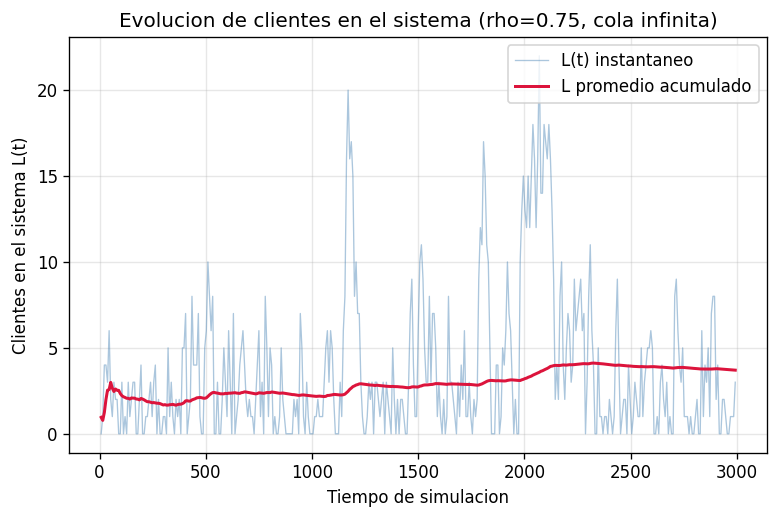
\includegraphics[width=0.7\textwidth]{output/L_evolucion_rho_0.75.png}
\caption{Evoluci\'on de la estimaci\'on acumulada de $L(t)$ para
$\rho = 0{,}75$. La estimaci\'on converge al valor te\'orico $L = 3$ a medida
que crece el horizonte de simulaci\'on.}
\label{fig:evolucion}
\end{figure}

\textbf{Medidas en funci\'on de la carga.} La Figura~\ref{fig:medidas}
agrupa las cuatro medidas de rendimiento en funci\'on de $\rho$, comparando
simulado y te\'orico. Se aprecia el crecimiento r\'apido (hiperb\'olico)
cerca de $\rho = 1$ y el ajuste estrecho en la zona estable.

\begin{figure}[H]
\centering
\begin{subfigure}{0.48\textwidth}
  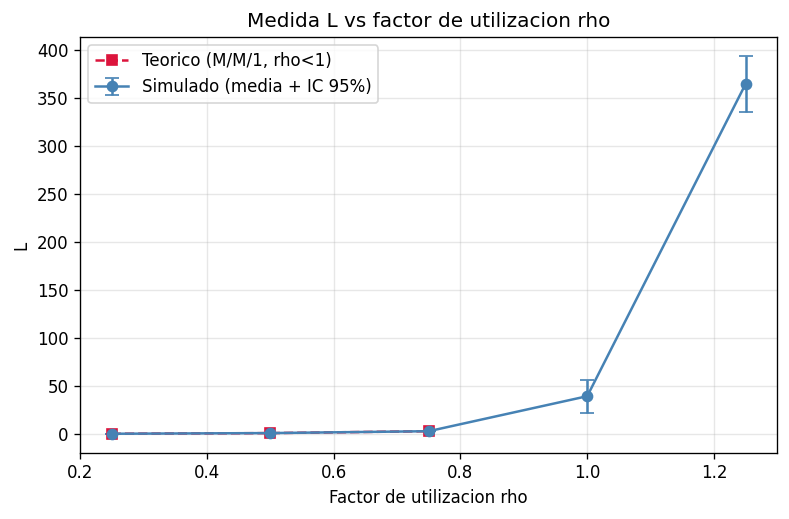
\includegraphics[width=\textwidth]{output/medida_L_vs_rho.png}
  \caption{$L$ (clientes en el sistema)}
\end{subfigure}
\begin{subfigure}{0.48\textwidth}
  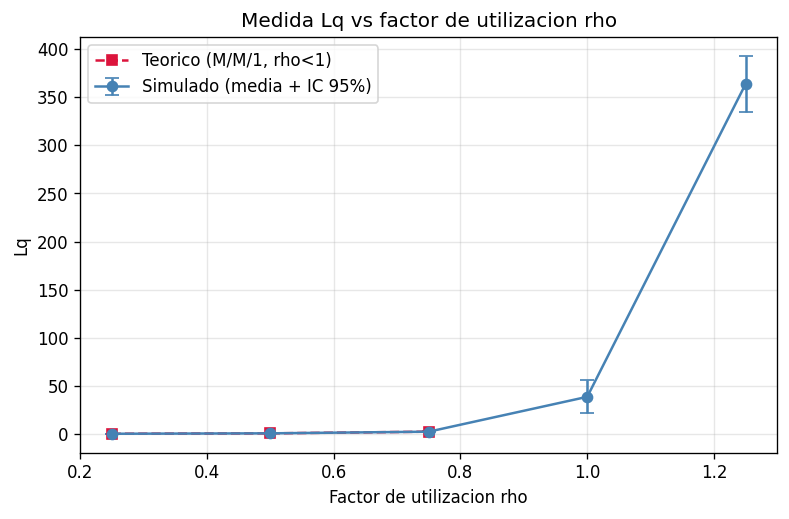
\includegraphics[width=\textwidth]{output/medida_Lq_vs_rho.png}
  \caption{$L_q$ (clientes en la cola)}
\end{subfigure}
\\[0.5em]
\begin{subfigure}{0.48\textwidth}
  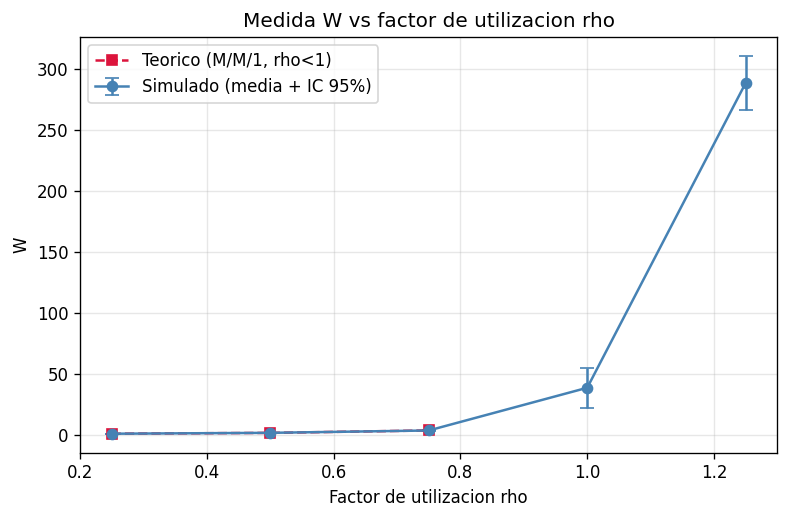
\includegraphics[width=\textwidth]{output/medida_W_vs_rho.png}
  \caption{$W$ (tiempo en el sistema)}
\end{subfigure}
\begin{subfigure}{0.48\textwidth}
  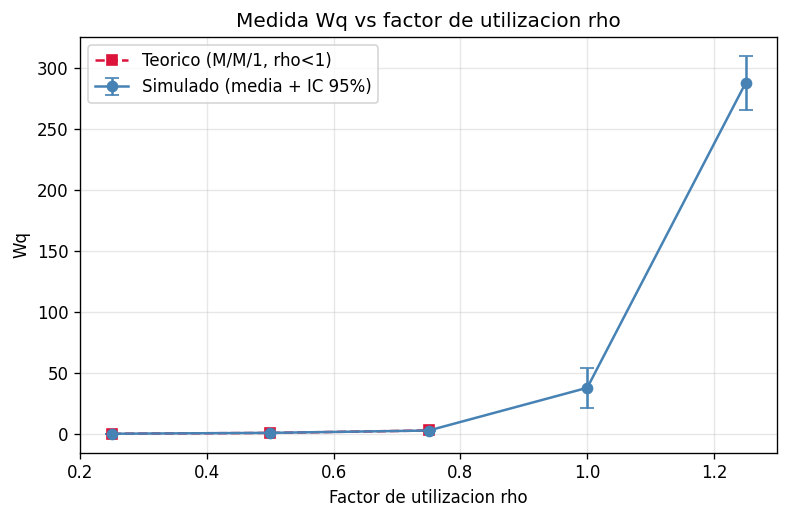
\includegraphics[width=\textwidth]{output/medida_Wq_vs_rho.png}
  \caption{$W_q$ (tiempo de espera en cola)}
\end{subfigure}
\caption{Medidas de rendimiento de la M/M/1 en funci\'on de la intensidad de
tr\'afico $\rho$: simulado vs.\ te\'orico. El ajuste es estrecho en la zona
estable y diverge al acercarse a $\rho = 1$.}
\label{fig:medidas}
\end{figure}

\textbf{Distribuci\'on estacionaria $P_n$.} La Figura~\ref{fig:pn} muestra
la distribuci\'on del n\'umero de clientes en el sistema (cola infinita) para
los tres niveles de carga estables, contrastando la frecuencia temporal
simulada con la geom\'etrica te\'orica $P_n = (1-\rho)\rho^n$.

\begin{figure}[H]
\centering
\begin{subfigure}{0.32\textwidth}
  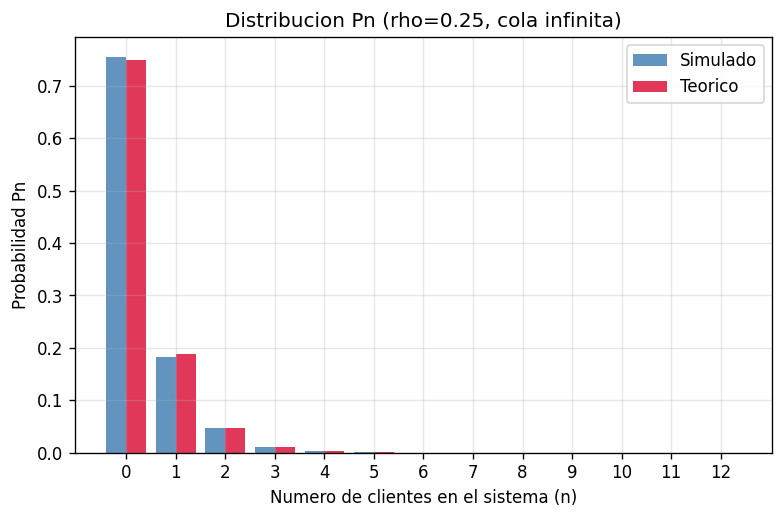
\includegraphics[width=\textwidth]{output/pn_infinita_rho_0.25.png}
  \caption{$\rho = 0{,}25$}
\end{subfigure}
\begin{subfigure}{0.32\textwidth}
  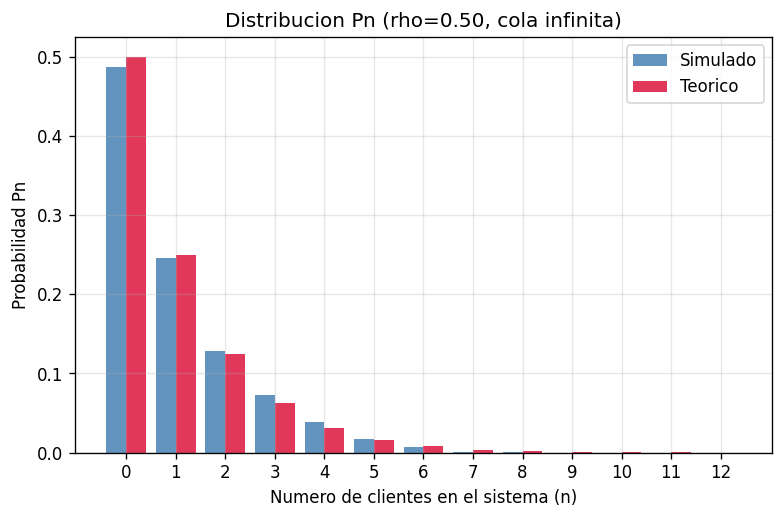
\includegraphics[width=\textwidth]{output/pn_infinita_rho_0.50.png}
  \caption{$\rho = 0{,}50$}
\end{subfigure}
\begin{subfigure}{0.32\textwidth}
  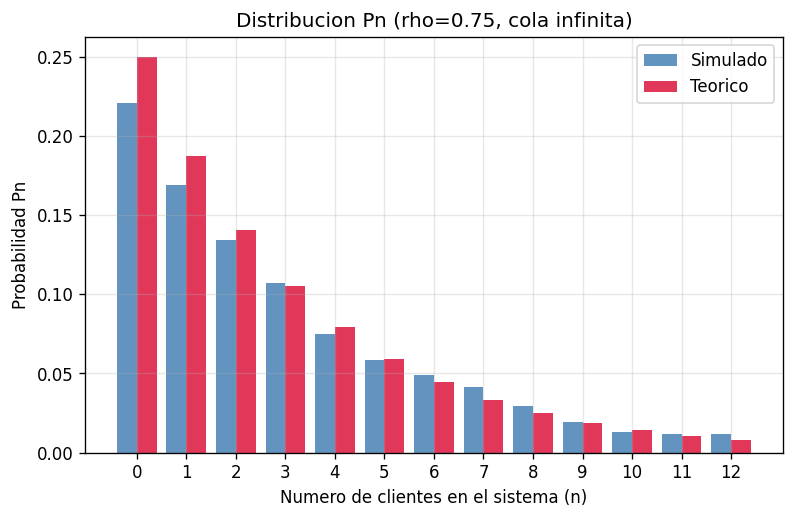
\includegraphics[width=\textwidth]{output/pn_infinita_rho_0.75.png}
  \caption{$\rho = 0{,}75$}
\end{subfigure}
\caption{Distribuci\'on estacionaria $P_n$ del n\'umero de clientes en la
M/M/1 infinita: fracci\'on de tiempo simulada (barras) vs.\ probabilidad
te\'orica $P_n = (1-\rho)\rho^n$ (puntos), para las tres cargas estables.}
\label{fig:pn}
\end{figure}

\textbf{Denegaci\'on en funci\'on de la capacidad.} La
Figura~\ref{fig:denegacion} resume c\'omo decae la probabilidad de
denegaci\'on al aumentar la capacidad $K$ de la cola finita, para los
distintos niveles de carga.

\begin{figure}[H]
\centering
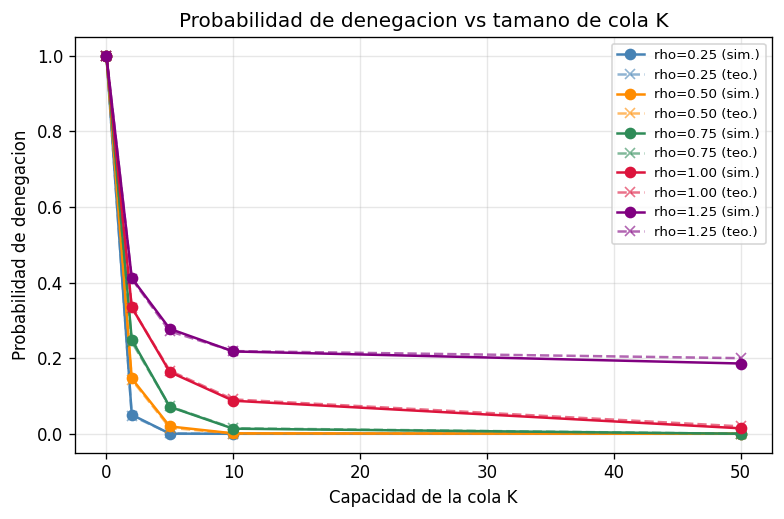
\includegraphics[width=0.7\textwidth]{output/denegacion_vs_K.png}
\caption{Probabilidad de denegaci\'on de la M/M/1/K en funci\'on de la
capacidad $K$, para cada nivel de carga $\rho$. La denegaci\'on decae
mon\'otonamente con $K$ y es mayor cuanto mayor es la carga.}
\label{fig:denegacion}
\end{figure}

\subsection{Comparaci\'on de fuentes: te\'orico / Python / AnyLogic}

El TP prev\'e contrastar \emph{tres} fuentes de datos independientes: el
valor te\'orico (f\'ormulas anal\'iticas), la simulaci\'on en Python (este
trabajo) y un modelo equivalente en \textbf{AnyLogic}. Se construy\'o en
AnyLogic el mismo sistema
Source~$\to$~Queue~$\to$~Service~$\to$~Sink con par\'ametros editables
($\lambda$, $\mu$, $K$) y se corri\'o un experimento Monte Carlo de $10$
r\'eplicas por cada nivel de carga $\rho$, con semillas aleatorias
independientes y horizonte $T = 5000$. El tiempo medio en el sistema $W$ se
ley\'o del histograma del experimento; las dem\'as medidas ($W_q$, $L$, $L_q$)
se derivaron mediante la ley de Little y la relaci\'on $W_q = W - 1/\mu$.
La Tabla~\ref{tab:fuentes} compara las tres fuentes para las cargas estables.

\begin{table}[H]
\centering
\small
\begin{tabular}{llrrr}
\toprule
\textbf{$\rho$} & \textbf{Medida} & \textbf{Te\'orico}
& \textbf{Python} & \textbf{AnyLogic} \\
\midrule
\multirow{4}{*}{$0{,}25$}
 & $L$   & $0{,}3333$ & $0{,}3365$ & $0{,}34$ \\
 & $L_q$ & $0{,}0833$ & $0{,}0847$ & $0{,}09$ \\
 & $W$   & $1{,}3333$ & $1{,}3260$ & $1{,}35$ \\
 & $W_q$ & $0{,}3333$ & $0{,}3335$ & $0{,}35$ \\
\midrule
\multirow{4}{*}{$0{,}50$}
 & $L$   & $1{,}0000$ & $1{,}0020$ & $0{,}99$ \\
 & $L_q$ & $0{,}5000$ & $0{,}5032$ & $0{,}49$ \\
 & $W$   & $2{,}0000$ & $2{,}0019$ & $1{,}98$ \\
 & $W_q$ & $1{,}0000$ & $1{,}0054$ & $0{,}98$ \\
\midrule
\multirow{4}{*}{$0{,}75$}
 & $L$   & $3{,}0000$ & $2{,}9631$ & $2{,}96$ \\
 & $L_q$ & $2{,}2500$ & $2{,}2146$ & $2{,}21$ \\
 & $W$   & $4{,}0000$ & $3{,}9442$ & $3{,}95$ \\
 & $W_q$ & $3{,}0000$ & $2{,}9473$ & $2{,}95$ \\
\bottomrule
\end{tabular}
\caption{Comparaci\'on de las tres fuentes (te\'orico / Python / AnyLogic)
para las cargas estables. La columna AnyLogic corresponde al promedio de $10$
r\'eplicas Monte Carlo en AnyLogic PLE con horizonte $T = 5000$; $W$ se
ley\'o del histograma y las dem\'as medidas se derivaron por ley de Little.}
\label{tab:fuentes}
\end{table}

\section{Discusi\'on}

\textbf{R\'egimen estable.} En la zona $\rho < 1$ el simulador reproduce la
teor\'ia con \'exito: para las tres cargas estables el error relativo
simulado--te\'orico es menor al $2\%$ en las cuatro medidas, y \emph{todos}
los intervalos de confianza al $95\%$ contienen al valor te\'orico
(Tabla~\ref{tab:infinita}). La utilizaci\'on observada $\hat{\rho}$ coincide
con $\rho = \lambda/\mu$ con error inferior al $1\%$, lo que confirma que el
generador de tiempos exponenciales y el motor de eventos est\'an bien
calibrados. La amplitud del intervalo de confianza crece con $\rho$ ---
mayor varianza entre r\'eplicas cuanto m\'as cargado el sistema ---, lo que es
esperable: cerca de la saturaci\'on el sistema es m\'as sensible a las
fluctuaciones de las semillas.

\textbf{R\'egimen inestable.} Para $\rho \ge 1$ la cola infinita es
\emph{inestable}: $L$ crece sin cota y s\'olo queda acotada por el horizonte
finito $T = 5000$. Los valores simulados ($L = 52{,}47$ para $\rho = 1$,
$L = 613{,}22$ para $\rho = 1{,}25$) no convergen a ning\'un l\'imite: son
artefactos del horizonte y crecer\'ian indefinidamente al extenderlo. Por eso
\emph{no} tiene sentido compararlos con la f\'ormula infinita (que da
$\infty$). El an\'alisis con significado en r\'egimen saturado se hace v\'ia la
\textbf{cola finita M/M/1/K}, que es \emph{siempre} estable porque la
capacidad acota el sistema, y donde la magnitud de inter\'es pasa a ser la
\emph{probabilidad de denegaci\'on}.

\textbf{Denegaci\'on.} La probabilidad de denegaci\'on simulada concuerda con
la te\'orica con error menor al $3\%$ en casi todos los casos
(Tabla~\ref{tab:denegacion}). Las \'unicas discrepancias relativas grandes
aparecen en denegaciones \emph{\'infimas} (del orden de $0{,}0005$, como en
$\rho = 0{,}50$, $K = 10$), donde el error relativo se infla simplemente
porque el denominador es diminuto; la diferencia \emph{absoluta} es
despreciable y carece de relevancia pr\'actica. El comportamiento cualitativo
es el esperado: la denegaci\'on crece con la carga $\rho$ y decae al
aumentar la capacidad $K$, hasta volverse pr\'acticamente nula para $K = 50$
salvo en sobrecarga ($\rho \ge 1$).

\textbf{Ley de Little como verificaci\'on cruzada.} Las medidas estimadas
satisfacen la ley de Little: por ejemplo, para $\rho = 0{,}50$ se tiene
$\lambda W = 0{,}5 \times 2{,}0019 = 1{,}0010 \approx L = 1{,}0020$, y
an\'alogamente $\lambda W_q \approx L_q$. Que la relaci\'on se cumpla
sirviendo de puente entre los promedios temporales ($L$, $L_q$) y los
promedios por cliente ($W$, $W_q$) --- estimados por v\'ias independientes
dentro del simulador --- es una validaci\'on interna fuerte de la coherencia
del motor.

\section{Conclusiones}

\begin{enumerate}
  \item Se construy\'o un simulador de eventos discretos de la cola M/M/1 (y
    su variante finita M/M/1/K) que, en r\'egimen estable ($\rho < 1$),
    reproduce las medidas te\'oricas $L$, $L_q$, $W$, $W_q$ y la
    utilizaci\'on con error menor al $2\%$, conteniendo siempre el valor
    te\'orico dentro del intervalo de confianza al $95\%$.
  \item En r\'egimen saturado ($\rho \ge 1$) la cola infinita es inestable y
    no admite comparaci\'on con la f\'ormula; el an\'alisis con sentido se
    traslada a la cola finita M/M/1/K, que es siempre estable.
  \item La probabilidad de denegaci\'on de servicio crece con la carga
    $\rho$ y decrece con la capacidad $K$, y el simulador la estima con error
    menor al $3\%$ salvo en denegaciones \'infimas, donde la diferencia
    absoluta es despreciable.
  \item El GCL validado en el TP 2.1, combinado con la transformaci\'on
    inversa para generar exponenciales, es una base de aleatoriedad
    suficiente para alimentar el simulador de colas.
  \item La tercera fuente de datos (AnyLogic, $10$ r\'eplicas Monte Carlo)
    confirma los resultados: las tres fuentes concuerdan con diferencias
    menores al $5\%$ en todas las medidas de la Tabla~\ref{tab:fuentes},
    validando el modelo desde tres perspectivas independientes.
\end{enumerate}

\begin{thebibliography}{9}

\bibitem{law}
Law, A. M. (2014). \emph{Simulation Modeling and Analysis}
(5\textsuperscript{a} ed.). McGraw-Hill.

\bibitem{kleinrock}
Kleinrock, L. (1975). \emph{Queueing Systems, Volume 1: Theory}.
Wiley-Interscience.

\bibitem{naylor}
Naylor, T. H. (1982). \emph{T\'ecnicas de simulaci\'on en computadoras}
(cap\'itulo 4: Generaci\'on de valores de las variables estoc\'asticas
empleadas en simulaci\'on). Limusa.

\bibitem{matplotlib}
Hunter, J. D. (2007). Matplotlib: A 2D Graphics Environment.
\emph{Computing in Science \& Engineering}, 9(3), 90-95.

\bibitem{python}
Van Rossum, G., \& Drake, F. L. (2009). \emph{Python 3 Reference Manual}.
CreateSpace.

\end{thebibliography}

\end{document}
